\documentclass[11pt]{article}

\usepackage{graphicx}
\usepackage{amsmath}
\usepackage{mathtools}
\usepackage{amssymb}
\usepackage[T1]{fontenc}
\usepackage[lithuanian]{babel}
\usepackage{listings}
\usepackage{subfigure}

\topmargin=-0.45in
\evensidemargin=0in
\oddsidemargin=0in
\textwidth=6.5in
\textheight=9.0in
\headsep=0.25in
    
\title{ Antras laboratorinis darbas}
\author{ Arnas Vaicekauskas }
\date{\today}

\begin{document}
\maketitle

\section{Uždavinys}

Išspręsti pirmos eilės diferencialinę lygtį su Koši pradine sąlyga naudojanti Rungės-Kuto 3-pakopį ir 4-pakopį skaitinius modelius.

\begin{align}
u'&=x+2x^2\sin(u)\\
u(0)&=-1
\end{align}

\section{Skaitiniai modeliai}

Skaitiniai modeliai įgyvendinti naudojant python programavimo kalbą, numpy ir scipy paketus.

\subsection{Rungė-Kuto 3-pakopis modelis}

\begin{align}
    \begin{cases}
        k_1&=f(x_n,y_n)\\
        k_2&=f(x_n+\tau,y_n+\tau k_1)\\
        k_3&=f(x_n+\frac{\tau}{2},y_n+\frac{\tau}{2}\frac{k_1+k_2}{2})\\
    \end{cases}\\
    y_{n+1}=y_n+\frac{\tau}{6}(k_1+k_2+4k_3).
\end{align}

\subsection{Rungė-Kuto 4-pakopis modelis}

\begin{align}
    \begin{cases}
        k_1&=f(x_n,y_n)\\
        k_2&=f(x_n+\frac{\tau}{2},y_n+\frac{\tau}{2}k_1)\\
        k_3&=f(x_n+\frac{\tau}{2},y_n+\frac{\tau}{2}k_2)\\
        k_4&=f(x_n+\tau,y_n+\tau k_3)\\
    \end{cases}\\
    y_{n+1}=y_n+\frac{\tau}{6}(k_1+2k_2+2k_3+k_4).
\end{align}

\newpage
\section{Rezultatai}

\subsection{Žymėjimas}

$x$ - laisvas kintamasis, 
$u_\tau$ - skaitinis sprendinys su žingsniu $\tau$,
$u_\tau(x)$ - skaitinio sprendinio su žingsniu $\tau$ reikšmė koordinatėje $x$,
$u(x)$ - analitinio sprendinio reikšmė koordinatėje $x$.

\subsection{Sprendinių grafikai}

\subsubsection{(a) dalis}

\begin{figure}[h!]
    \centering
    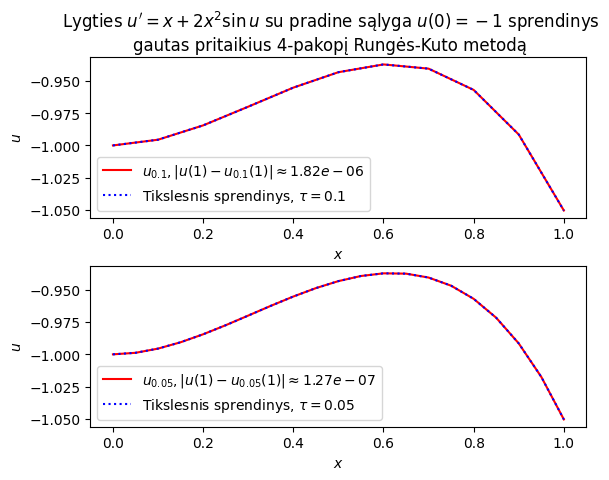
\includegraphics[width=0.8\textwidth]{a1.png}
    \caption{Skaitiniai lygties sprendiniai, kai $\tau=0.1, 0.05$ lyginami su tikslesniu sprendiniu gautu naudojant scipy metodą odeint.}
    \label{fig:pvz1}
\end{figure}

\newpage
\subsubsection{(b) dalis}

\begin{figure}[h!]
    \centering
    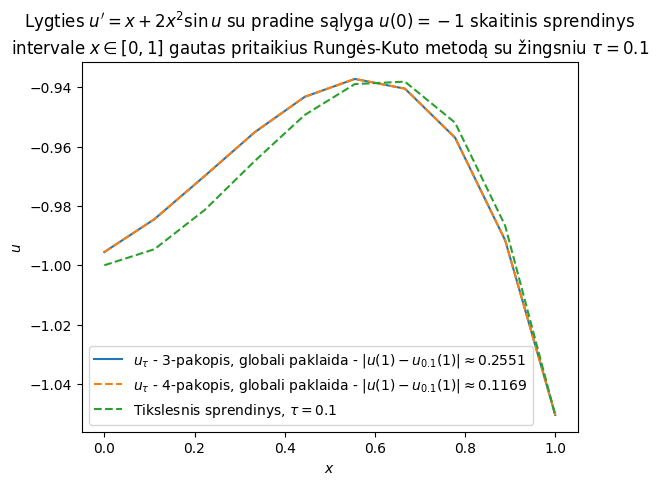
\includegraphics[width=0.8\textwidth]{b1.png}
    \caption{Skaitiniai lygties sprendiniai gauti skirtingais metodais lyginami su tikslesniu sprendiniu gautu naudojant scipy metodą odeint.}
    \label{fig:pvz2}
\end{figure}

\newpage
\subsection{Paklaidos vertinimas}

Rungės metodas paklaidai įvertinti

\begin{align}
\vert u(x)-u_{\tau}(x)\vert\approx\frac{\vert u_{2\tau}(x) - u_{\tau}(x)\vert}{2^p - 1}
\end{align}

\begin{figure}[h!]
    \centering
    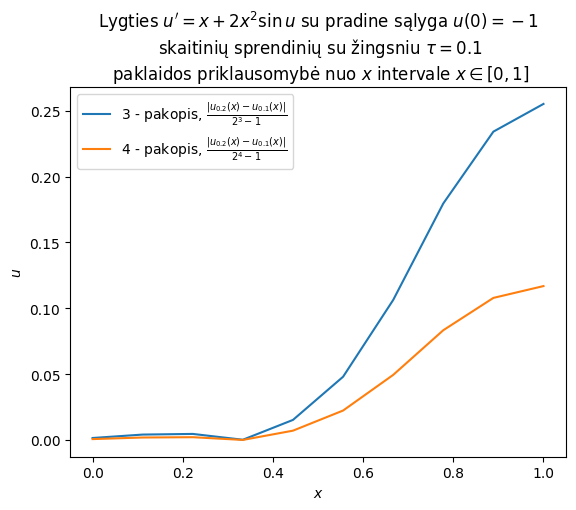
\includegraphics[width=0.8\textwidth]{error.png}
    \caption{Skaitinių metodų paklaidos.}
    \label{fig:pvz3}
\end{figure}

\newpage
\section{Priedai}

Programos kodas naudotas sugeneruoti visus šiame dokumente esančius grafikus. Kode naudojamos antraštės išimtos, nes
netelpa dokumente ir LaTeX kompiliatorius nesugeba sukompiliuoti simbolių eilučių, kuriose yra LaTeX kodo. 

\begin{lstlisting}[language=Python]
import numpy as np
from scipy.integrate import odeint
import matplotlib.pyplot as plt

def rk3(f, t_0, y_0, tau, N):
    t_current = t_0
    y_current = y_0

    ys = np.zeros(N)

    for i in range(N):
        k1 = f(t_current, y_current)
        k2 = f(t_current + tau, y_current + tau * k1)
        k3 = f(t_current + tau/2, y_current + tau/2 * (k1 + k2)/2 )
        
        t_current = t_current + tau
        y_current = y_current + tau/6 * (k1 + k2 + 4*k3)
        ys[i] = y_current
    return ys

def rk4(f, t_0, y_0, tau, N):

    t_current = t_0
    y_current = y_0

    ys = np.zeros(N)

    for i in range(N):
        k1 = f(t_current, y_current)
        k2 = f(t_current + tau/2, y_current + tau/2 * k1)
        k3 = f(t_current + tau/2, y_current + tau/2 * k2)
        k4 = f(t_current + tau, y_current + tau * k3)

        t_current = t_current + tau
        y_current = y_current + tau/6 * (k1 + 2*k2 + 2*k3 + k4)
        ys[i] = y_current
    return ys

def f(t, u):
    return t + 2 * t**2 * np.sin(u)

u_0 = -1
x_0 = 0
x_end = 1
tau = [0.1, 0.05]

plt.xlabel('$x$')
plt.ylabel('$u$')

fig, axes = plt.subplots(2, sharey=True)

for index, tau_i in enumerate(tau):
    if index == 0:
        axes[index].set_title("")
    N = int((x_end - x_0) / tau_i)
    xs = np.linspace(x_0, 1, N)
    us = rk4(f, x_0, u_0, tau_i, N)
    us_real = odeint(lambda u, t: f(t, u), u_0, xs)
    axes[index].plot(xs, us_real,label="", linestyle='dashed')
    us_double_tau = rk4(f, x_0, u_0, 2 * tau_i, N)
    error = np.abs(us_double_tau[-1] - us[-1]) / (2**4 - 1)
    label = ""
    axes[index].plot(xs, us, label=label)
    axes[index].legend()
plt.show()

tau = 0.1
plt.title("")
plt.xlabel("")
plt.ylabel("")

N = int((x_end - x_0) / tau)
xs = np.linspace(x_0, 1, N)

us_3 = rk3(f, x_0, u_0, tau, N)
us_4 = rk4(f, x_0, u_0, tau, N)

us_3_double_tau = rk3(f, x_0, u_0, 2 * tau, N)
us_4_double_tau = rk4(f, x_0, u_0, 2 * tau, N)

error_3_global = np.abs(us_3_double_tau[-1] - us_3[-1]) / (2**3 - 1)
error_4_global = np.abs(us_4_double_tau[-1] - us_4[-1]) / (2**4 - 1)

label = ""
plt.plot(xs, us_3, label=label)

label = ""
plt.plot(xs, us_4, label=label, linestyle='dashed')
    
us_real = odeint(lambda u, t: f(t, u), u_0, xs)
plt.plot(xs, us_real,label="", linestyle='dashed')

plt.legend()
plt.show()
    
error_3_local = np.abs(us_3_double_tau - us_3) / (2**3 - 1)
error_4_local = np.abs(us_4_double_tau - us_4) / (2**4 - 1)

plt.title("")
label = ""
plt.plot(xs, error_3_local, label=label)
label = ""
plt.plot(xs, error_4_local, label=label)
plt.legend()
plt.xlabel("")
plt.ylabel("")
plt.show()
\end{lstlisting}

\end{document}